\section{Implementation}

\begin{itemize}[noitemsep]
   \item	Installation von 3 VMs
   \begin{enumerate}[noitemsep]
      \item Grafana
      \item Normal user
      \item Angreifer
   \end{enumerate}
   \item	Diagramm der Struktur
\end{itemize}

\subsection{Angriffe}
Erklärung wie die Angriffe funktionieren nach \gls{mitre}.
SSH-BruteForce
Diagramm des Angriffes

\subsection{Bewertung der Daten in Grafana}
Hinzufügen der Logdateien und Erstellung von Regeln zur Erkennung des Angriffes
Diagramm der Nutzung von Grafana

\subsection{Normalisierung der Logdateien mit Zeek}
Diagramm der Nutzung von Grafana und Zeek

Hier werden die Schritte für die Installation und Sammeln von Daten beschrieben.

- Implementation in Container %https://rdr-it.com/elk-installation-configuration-un-siem-docker/
\begin{figure}[H]
   \centering
   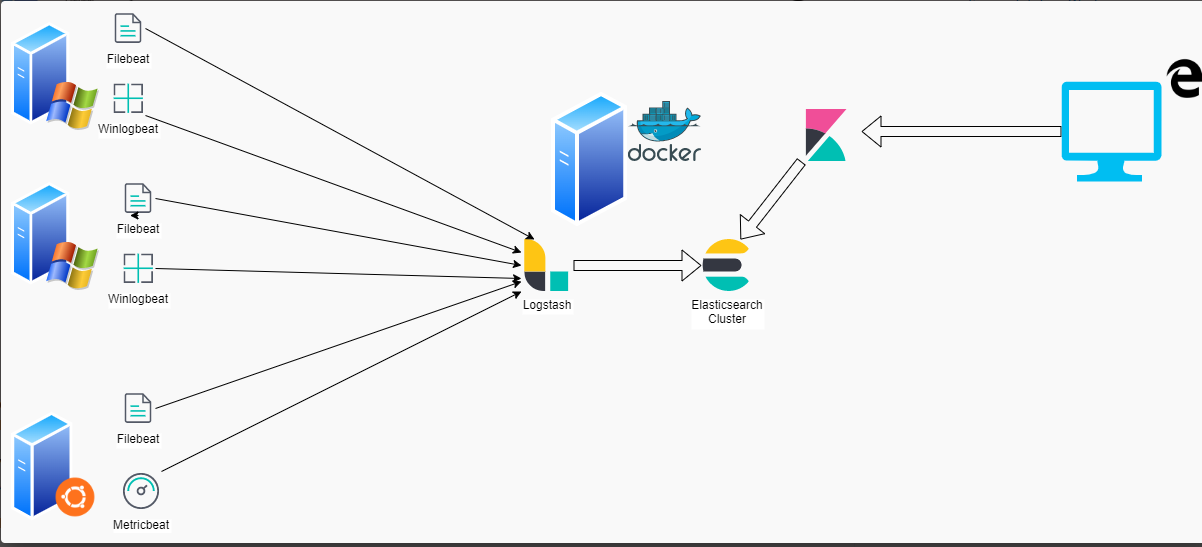
\includegraphics[width=0.8\textwidth]{assets/3_p1.png}
   \caption{Struktur von \gls{SIEM} in einem Container \\Quelle: \citep{RDR_Docker}}
   \centering
\end{figure}


\subsection{Sammlung von Server-Log Dateien}

\subsection{Normalisierung der Log-Dateien}





